\documentclass[twoside]{book}

% Packages required by doxygen
\usepackage{fixltx2e}
\usepackage{calc}
\usepackage{doxygen}
\usepackage[export]{adjustbox} % also loads graphicx
\usepackage{graphicx}
\usepackage[utf8]{inputenc}
\usepackage{makeidx}
\usepackage{multicol}
\usepackage{multirow}
\PassOptionsToPackage{warn}{textcomp}
\usepackage{textcomp}
\usepackage[nointegrals]{wasysym}
\usepackage[table]{xcolor}

% NLS support packages
\usepackage[T2A]{fontenc}
\usepackage[russian]{babel}

% Font selection
\usepackage[T1]{fontenc}
\usepackage[scaled=.90]{helvet}
\usepackage{courier}
\usepackage{amssymb}
\usepackage{sectsty}
\renewcommand{\familydefault}{\sfdefault}
\allsectionsfont{%
  \fontseries{bc}\selectfont%
  \color{darkgray}%
}
\renewcommand{\DoxyLabelFont}{%
  \fontseries{bc}\selectfont%
  \color{darkgray}%
}
\newcommand{\+}{\discretionary{\mbox{\scriptsize$\hookleftarrow$}}{}{}}

% Page & text layout
\usepackage{geometry}
\geometry{%
  a4paper,%
  top=2.5cm,%
  bottom=2.5cm,%
  left=2.5cm,%
  right=2.5cm%
}
\tolerance=750
\hfuzz=15pt
\hbadness=750
\setlength{\emergencystretch}{15pt}
\setlength{\parindent}{0cm}
\setlength{\parskip}{3ex plus 2ex minus 2ex}
\makeatletter
\renewcommand{\paragraph}{%
  \@startsection{paragraph}{4}{0ex}{-1.0ex}{1.0ex}{%
    \normalfont\normalsize\bfseries\SS@parafont%
  }%
}
\renewcommand{\subparagraph}{%
  \@startsection{subparagraph}{5}{0ex}{-1.0ex}{1.0ex}{%
    \normalfont\normalsize\bfseries\SS@subparafont%
  }%
}
\makeatother

% Headers & footers
\usepackage{fancyhdr}
\pagestyle{fancyplain}
\fancyhead[LE]{\fancyplain{}{\bfseries\thepage}}
\fancyhead[CE]{\fancyplain{}{}}
\fancyhead[RE]{\fancyplain{}{\bfseries\leftmark}}
\fancyhead[LO]{\fancyplain{}{\bfseries\rightmark}}
\fancyhead[CO]{\fancyplain{}{}}
\fancyhead[RO]{\fancyplain{}{\bfseries\thepage}}
\fancyfoot[LE]{\fancyplain{}{}}
\fancyfoot[CE]{\fancyplain{}{}}
\fancyfoot[RE]{\fancyplain{}{\bfseries\scriptsize Создано системой Doxygen }}
\fancyfoot[LO]{\fancyplain{}{\bfseries\scriptsize Создано системой Doxygen }}
\fancyfoot[CO]{\fancyplain{}{}}
\fancyfoot[RO]{\fancyplain{}{}}
\renewcommand{\footrulewidth}{0.4pt}
\renewcommand{\chaptermark}[1]{%
  \markboth{#1}{}%
}
\renewcommand{\sectionmark}[1]{%
  \markright{\thesection\ #1}%
}

% Indices & bibliography
\usepackage{natbib}
\usepackage[titles]{tocloft}
\setcounter{tocdepth}{3}
\setcounter{secnumdepth}{5}
\makeindex

% Hyperlinks (required, but should be loaded last)
\usepackage{ifpdf}
\ifpdf
  \usepackage[pdftex,pagebackref=true]{hyperref}
\else
  \usepackage[ps2pdf,pagebackref=true]{hyperref}
\fi
\hypersetup{%
  colorlinks=true,%
  linkcolor=blue,%
  citecolor=blue,%
  unicode%
}

% Custom commands
\newcommand{\clearemptydoublepage}{%
  \newpage{\pagestyle{empty}\cleardoublepage}%
}

\usepackage{caption}
\captionsetup{labelsep=space,justification=centering,font={bf},singlelinecheck=off,skip=4pt,position=top}

%===== C O N T E N T S =====

\begin{document}

% Titlepage & ToC
\hypersetup{pageanchor=false,
             bookmarksnumbered=true,
             pdfencoding=unicode
            }
\pagenumbering{alph}
\begin{titlepage}
\vspace*{7cm}
\begin{center}%
{\Large Daily\+Actions\+Tracker }\\
\vspace*{1cm}
{\large Создано системой Doxygen 1.8.14}\\
\end{center}
\end{titlepage}
\clearemptydoublepage
\pagenumbering{roman}
\tableofcontents
\clearemptydoublepage
\pagenumbering{arabic}
\hypersetup{pageanchor=true}

%--- Begin generated contents ---
\chapter{Алфавитный указатель пространств имен}
\section{Пакеты}
Полный список документированных пакетов.\begin{DoxyCompactList}
\item\contentsline{section}{\mbox{\hyperlink{namespaceapp}{app}} }{\pageref{namespaceapp}}{}
\item\contentsline{section}{\mbox{\hyperlink{namespaceapp_1_1errors}{app.\+errors}} }{\pageref{namespaceapp_1_1errors}}{}
\item\contentsline{section}{\mbox{\hyperlink{namespaceapp_1_1forms}{app.\+forms}} }{\pageref{namespaceapp_1_1forms}}{}
\item\contentsline{section}{\mbox{\hyperlink{namespaceapp_1_1logger}{app.\+logger}} }{\pageref{namespaceapp_1_1logger}}{}
\item\contentsline{section}{\mbox{\hyperlink{namespaceapp_1_1models}{app.\+models}} }{\pageref{namespaceapp_1_1models}}{}
\item\contentsline{section}{\mbox{\hyperlink{namespaceapp_1_1routes}{app.\+routes}} }{\pageref{namespaceapp_1_1routes}}{}
\end{DoxyCompactList}

\chapter{Иерархический список классов}
\section{Иерархия классов}
Иерархия классов.\begin{DoxyCompactList}
\item Model\begin{DoxyCompactList}
\item \contentsline{section}{app.\+models.\+Task}{\pageref{classapp_1_1models_1_1_task}}{}
\item \contentsline{section}{app.\+models.\+User}{\pageref{classapp_1_1models_1_1_user}}{}
\end{DoxyCompactList}
\item Flask\+Form\begin{DoxyCompactList}
\item \contentsline{section}{app.\+forms.\+Add\+Task\+Form}{\pageref{classapp_1_1forms_1_1_add_task_form}}{}
\item \contentsline{section}{app.\+forms.\+Edit\+Profile\+Form}{\pageref{classapp_1_1forms_1_1_edit_profile_form}}{}
\item \contentsline{section}{app.\+forms.\+Login\+Form}{\pageref{classapp_1_1forms_1_1_login_form}}{}
\item \contentsline{section}{app.\+forms.\+Registration\+Form}{\pageref{classapp_1_1forms_1_1_registration_form}}{}
\end{DoxyCompactList}
\item User\+Mixin\begin{DoxyCompactList}
\item \contentsline{section}{app.\+models.\+User}{\pageref{classapp_1_1models_1_1_user}}{}
\end{DoxyCompactList}
\end{DoxyCompactList}

\chapter{Алфавитный указатель классов}
\section{Классы}
Классы с их кратким описанием.\begin{DoxyCompactList}
\item\contentsline{section}{\mbox{\hyperlink{classapp_1_1forms_1_1_add_task_form}{app.\+forms.\+Add\+Task\+Form}} \\*Класс формы добавления активности/задачи }{\pageref{classapp_1_1forms_1_1_add_task_form}}{}
\item\contentsline{section}{\mbox{\hyperlink{classapp_1_1forms_1_1_edit_profile_form}{app.\+forms.\+Edit\+Profile\+Form}} \\*Класс формы редактирования профиля }{\pageref{classapp_1_1forms_1_1_edit_profile_form}}{}
\item\contentsline{section}{\mbox{\hyperlink{classapp_1_1forms_1_1_login_form}{app.\+forms.\+Login\+Form}} \\*Класс формы входа }{\pageref{classapp_1_1forms_1_1_login_form}}{}
\item\contentsline{section}{\mbox{\hyperlink{classapp_1_1forms_1_1_registration_form}{app.\+forms.\+Registration\+Form}} \\*Класс формы регистрации }{\pageref{classapp_1_1forms_1_1_registration_form}}{}
\item\contentsline{section}{\mbox{\hyperlink{classapp_1_1models_1_1_task}{app.\+models.\+Task}} \\*Класс активностей }{\pageref{classapp_1_1models_1_1_task}}{}
\item\contentsline{section}{\mbox{\hyperlink{classapp_1_1models_1_1_user}{app.\+models.\+User}} \\*Класс пользователей }{\pageref{classapp_1_1models_1_1_user}}{}
\end{DoxyCompactList}

\chapter{Список файлов}
\section{Файлы}
Полный список файлов.\begin{DoxyCompactList}
\item\contentsline{section}{app/\mbox{\hyperlink{____init_____8py}{\+\_\+\+\_\+init\+\_\+\+\_\+.\+py}} }{\pageref{____init_____8py}}{}
\item\contentsline{section}{app/\mbox{\hyperlink{errors_8py}{errors.\+py}} }{\pageref{errors_8py}}{}
\item\contentsline{section}{app/\mbox{\hyperlink{forms_8py}{forms.\+py}} }{\pageref{forms_8py}}{}
\item\contentsline{section}{app/\mbox{\hyperlink{logger_8py}{logger.\+py}} }{\pageref{logger_8py}}{}
\item\contentsline{section}{app/\mbox{\hyperlink{models_8py}{models.\+py}} }{\pageref{models_8py}}{}
\item\contentsline{section}{app/\mbox{\hyperlink{routes_8py}{routes.\+py}} }{\pageref{routes_8py}}{}
\end{DoxyCompactList}

\chapter{Пространства имен}
\hypertarget{namespaceapp}{}\section{Пространство имен app}
\label{namespaceapp}\index{app@{app}}
\subsection*{Пространства имен}
\begin{DoxyCompactItemize}
\item 
 \mbox{\hyperlink{namespaceapp_1_1errors}{errors}}
\item 
 \mbox{\hyperlink{namespaceapp_1_1forms}{forms}}
\item 
 \mbox{\hyperlink{namespaceapp_1_1logger}{logger}}
\item 
 \mbox{\hyperlink{namespaceapp_1_1models}{models}}
\item 
 \mbox{\hyperlink{namespaceapp_1_1routes}{routes}}
\end{DoxyCompactItemize}
\subsection*{Переменные}
\begin{DoxyCompactItemize}
\item 
\mbox{\hyperlink{namespaceapp_a675b4ea702c13dc4b8c05f985a25b496}{app}} = Flask(\+\_\+\+\_\+name\+\_\+\+\_\+)
\item 
\mbox{\hyperlink{namespaceapp_a75341a4bc0e8e239f299316136af3466}{db}} = S\+Q\+L\+Alchemy(\mbox{\hyperlink{namespaceapp_a675b4ea702c13dc4b8c05f985a25b496}{app}})
\item 
\mbox{\hyperlink{namespaceapp_a15a40303715f32fc22108c84baaeb68d}{migrate}} = Migrate(\mbox{\hyperlink{namespaceapp_a675b4ea702c13dc4b8c05f985a25b496}{app}}, \mbox{\hyperlink{namespaceapp_a75341a4bc0e8e239f299316136af3466}{db}})
\item 
\mbox{\hyperlink{namespaceapp_ab9cb25b758b83ccf851448416d009420}{login}} = Login\+Manager(\mbox{\hyperlink{namespaceapp_a675b4ea702c13dc4b8c05f985a25b496}{app}})
\item 
\mbox{\hyperlink{namespaceapp_a0cbb607dd84c52fec23f2a56b7151163}{login\+\_\+view}}
\item 
\mbox{\hyperlink{namespaceapp_ab0100f0fe587f9be45118e0ab4c7dc32}{bootstrap}} = Bootstrap(\mbox{\hyperlink{namespaceapp_a675b4ea702c13dc4b8c05f985a25b496}{app}})
\end{DoxyCompactItemize}


\subsection{Переменные}
\mbox{\Hypertarget{namespaceapp_a675b4ea702c13dc4b8c05f985a25b496}\label{namespaceapp_a675b4ea702c13dc4b8c05f985a25b496}} 
\index{app@{app}!app@{app}}
\index{app@{app}!app@{app}}
\subsubsection{\texorpdfstring{app}{app}}
{\footnotesize\ttfamily app.\+app = Flask(\+\_\+\+\_\+name\+\_\+\+\_\+)}

\mbox{\Hypertarget{namespaceapp_ab0100f0fe587f9be45118e0ab4c7dc32}\label{namespaceapp_ab0100f0fe587f9be45118e0ab4c7dc32}} 
\index{app@{app}!bootstrap@{bootstrap}}
\index{bootstrap@{bootstrap}!app@{app}}
\subsubsection{\texorpdfstring{bootstrap}{bootstrap}}
{\footnotesize\ttfamily app.\+bootstrap = Bootstrap(\mbox{\hyperlink{namespaceapp_a675b4ea702c13dc4b8c05f985a25b496}{app}})}

\mbox{\Hypertarget{namespaceapp_a75341a4bc0e8e239f299316136af3466}\label{namespaceapp_a75341a4bc0e8e239f299316136af3466}} 
\index{app@{app}!db@{db}}
\index{db@{db}!app@{app}}
\subsubsection{\texorpdfstring{db}{db}}
{\footnotesize\ttfamily app.\+db = S\+Q\+L\+Alchemy(\mbox{\hyperlink{namespaceapp_a675b4ea702c13dc4b8c05f985a25b496}{app}})}

\mbox{\Hypertarget{namespaceapp_ab9cb25b758b83ccf851448416d009420}\label{namespaceapp_ab9cb25b758b83ccf851448416d009420}} 
\index{app@{app}!login@{login}}
\index{login@{login}!app@{app}}
\subsubsection{\texorpdfstring{login}{login}}
{\footnotesize\ttfamily app.\+login = Login\+Manager(\mbox{\hyperlink{namespaceapp_a675b4ea702c13dc4b8c05f985a25b496}{app}})}

\mbox{\Hypertarget{namespaceapp_a0cbb607dd84c52fec23f2a56b7151163}\label{namespaceapp_a0cbb607dd84c52fec23f2a56b7151163}} 
\index{app@{app}!login\+\_\+view@{login\+\_\+view}}
\index{login\+\_\+view@{login\+\_\+view}!app@{app}}
\subsubsection{\texorpdfstring{login\+\_\+view}{login\_view}}
{\footnotesize\ttfamily app.\+login\+\_\+view}

\mbox{\Hypertarget{namespaceapp_a15a40303715f32fc22108c84baaeb68d}\label{namespaceapp_a15a40303715f32fc22108c84baaeb68d}} 
\index{app@{app}!migrate@{migrate}}
\index{migrate@{migrate}!app@{app}}
\subsubsection{\texorpdfstring{migrate}{migrate}}
{\footnotesize\ttfamily app.\+migrate = Migrate(\mbox{\hyperlink{namespaceapp_a675b4ea702c13dc4b8c05f985a25b496}{app}}, \mbox{\hyperlink{namespaceapp_a75341a4bc0e8e239f299316136af3466}{db}})}


\hypertarget{namespaceapp_1_1errors}{}\section{Пространство имен app.\+errors}
\label{namespaceapp_1_1errors}\index{app.\+errors@{app.\+errors}}
\subsection*{Функции}
\begin{DoxyCompactItemize}
\item 
def \mbox{\hyperlink{namespaceapp_1_1errors_a9194a32acf0c07060c8375e17f202af8}{not\+\_\+found\+\_\+error}} (error)
\begin{DoxyCompactList}\small\item\em Обработчик ошибки 404 \char`\"{}\+File not found\char`\"{}. \end{DoxyCompactList}\item 
def \mbox{\hyperlink{namespaceapp_1_1errors_a080d04aef974075b9be3ed7f6e45d73a}{internal\+\_\+error}} (error)
\begin{DoxyCompactList}\small\item\em Обработчик ошибки 500. \end{DoxyCompactList}\end{DoxyCompactItemize}


\subsection{Функции}
\mbox{\Hypertarget{namespaceapp_1_1errors_a080d04aef974075b9be3ed7f6e45d73a}\label{namespaceapp_1_1errors_a080d04aef974075b9be3ed7f6e45d73a}} 
\index{app\+::errors@{app\+::errors}!internal\+\_\+error@{internal\+\_\+error}}
\index{internal\+\_\+error@{internal\+\_\+error}!app\+::errors@{app\+::errors}}
\subsubsection{\texorpdfstring{internal\+\_\+error()}{internal\_error()}}
{\footnotesize\ttfamily def app.\+errors.\+internal\+\_\+error (\begin{DoxyParamCaption}\item[{}]{error }\end{DoxyParamCaption})}



Обработчик ошибки 500. 


\begin{DoxyParams}{Аргументы}
{\em error} & -\/ код ошибки \\
\hline
\end{DoxyParams}
\begin{DoxyReturn}{Возвращает}
страницу с ошибкой (500.\+html) 
\end{DoxyReturn}
\mbox{\Hypertarget{namespaceapp_1_1errors_a9194a32acf0c07060c8375e17f202af8}\label{namespaceapp_1_1errors_a9194a32acf0c07060c8375e17f202af8}} 
\index{app\+::errors@{app\+::errors}!not\+\_\+found\+\_\+error@{not\+\_\+found\+\_\+error}}
\index{not\+\_\+found\+\_\+error@{not\+\_\+found\+\_\+error}!app\+::errors@{app\+::errors}}
\subsubsection{\texorpdfstring{not\+\_\+found\+\_\+error()}{not\_found\_error()}}
{\footnotesize\ttfamily def app.\+errors.\+not\+\_\+found\+\_\+error (\begin{DoxyParamCaption}\item[{}]{error }\end{DoxyParamCaption})}



Обработчик ошибки 404 \char`\"{}\+File not found\char`\"{}. 


\begin{DoxyParams}{Аргументы}
{\em error} & -\/ код ошибки \\
\hline
\end{DoxyParams}
\begin{DoxyReturn}{Возвращает}
страницу с ошибкой (404.\+html) 
\end{DoxyReturn}

\hypertarget{namespaceapp_1_1forms}{}\section{Пространство имен app.\+forms}
\label{namespaceapp_1_1forms}\index{app.\+forms@{app.\+forms}}
\subsection*{Классы}
\begin{DoxyCompactItemize}
\item 
class \mbox{\hyperlink{classapp_1_1forms_1_1_add_task_form}{Add\+Task\+Form}}
\begin{DoxyCompactList}\small\item\em Класс формы добавления активности/задачи \end{DoxyCompactList}\item 
class \mbox{\hyperlink{classapp_1_1forms_1_1_edit_profile_form}{Edit\+Profile\+Form}}
\begin{DoxyCompactList}\small\item\em Класс формы редактирования профиля \end{DoxyCompactList}\item 
class \mbox{\hyperlink{classapp_1_1forms_1_1_login_form}{Login\+Form}}
\begin{DoxyCompactList}\small\item\em Класс формы входа \end{DoxyCompactList}\item 
class \mbox{\hyperlink{classapp_1_1forms_1_1_registration_form}{Registration\+Form}}
\begin{DoxyCompactList}\small\item\em Класс формы регистрации \end{DoxyCompactList}\end{DoxyCompactItemize}

\hypertarget{namespaceapp_1_1logger}{}\section{Пространство имен app.\+logger}
\label{namespaceapp_1_1logger}\index{app.\+logger@{app.\+logger}}
\subsection*{Переменные}
\begin{DoxyCompactItemize}
\item 
\mbox{\hyperlink{namespaceapp_1_1logger_ad08dccf52a81966328998e474ec1b933}{file\+\_\+handler}}
\end{DoxyCompactItemize}


\subsection{Переменные}
\mbox{\Hypertarget{namespaceapp_1_1logger_ad08dccf52a81966328998e474ec1b933}\label{namespaceapp_1_1logger_ad08dccf52a81966328998e474ec1b933}} 
\index{app\+::logger@{app\+::logger}!file\+\_\+handler@{file\+\_\+handler}}
\index{file\+\_\+handler@{file\+\_\+handler}!app\+::logger@{app\+::logger}}
\subsubsection{\texorpdfstring{file\+\_\+handler}{file\_handler}}
{\footnotesize\ttfamily app.\+logger.\+file\+\_\+handler}

{\bfseries Инициализатор}
\begin{DoxyCode}
1 =  RotatingFileHandler(\textcolor{stringliteral}{'logs/project.log'}, maxBytes=10240,
2                                        backupCount=10)
\end{DoxyCode}

\hypertarget{namespaceapp_1_1models}{}\section{Пространство имен app.\+models}
\label{namespaceapp_1_1models}\index{app.\+models@{app.\+models}}
\subsection*{Классы}
\begin{DoxyCompactItemize}
\item 
class \mbox{\hyperlink{classapp_1_1models_1_1_task}{Task}}
\begin{DoxyCompactList}\small\item\em Класс активностей \end{DoxyCompactList}\item 
class \mbox{\hyperlink{classapp_1_1models_1_1_user}{User}}
\begin{DoxyCompactList}\small\item\em Класс пользователей \end{DoxyCompactList}\end{DoxyCompactItemize}
\subsection*{Функции}
\begin{DoxyCompactItemize}
\item 
def \mbox{\hyperlink{namespaceapp_1_1models_a3d862de59e8282c7b45881c299a9266d}{load\+\_\+user}} (id)
\begin{DoxyCompactList}\small\item\em Загрузка Пользователя \end{DoxyCompactList}\end{DoxyCompactItemize}


\subsection{Функции}
\mbox{\Hypertarget{namespaceapp_1_1models_a3d862de59e8282c7b45881c299a9266d}\label{namespaceapp_1_1models_a3d862de59e8282c7b45881c299a9266d}} 
\index{app\+::models@{app\+::models}!load\+\_\+user@{load\+\_\+user}}
\index{load\+\_\+user@{load\+\_\+user}!app\+::models@{app\+::models}}
\subsubsection{\texorpdfstring{load\+\_\+user()}{load\_user()}}
{\footnotesize\ttfamily def app.\+models.\+load\+\_\+user (\begin{DoxyParamCaption}\item[{}]{id }\end{DoxyParamCaption})}



Загрузка Пользователя 


\begin{DoxyParams}{Аргументы}
{\em id} & -\/ первичный ключ пользователя \\
\hline
\end{DoxyParams}

\hypertarget{namespaceapp_1_1routes}{}\section{Пространство имен app.\+routes}
\label{namespaceapp_1_1routes}\index{app.\+routes@{app.\+routes}}
\subsection*{Функции}
\begin{DoxyCompactItemize}
\item 
def \mbox{\hyperlink{namespaceapp_1_1routes_a724739005fa07eb8591ce53b0daf3dc1}{index}} ()
\begin{DoxyCompactList}\small\item\em Обработчик маршрута главной страницы (index). \end{DoxyCompactList}\item 
def \mbox{\hyperlink{namespaceapp_1_1routes_a55242b1fcb58ff44c5b793cbb5335272}{login}} ()
\begin{DoxyCompactList}\small\item\em Обработчик маршрута страницы входа (login). \end{DoxyCompactList}\item 
def \mbox{\hyperlink{namespaceapp_1_1routes_a3031cfc20f4e9f9624a1a7351483fcb3}{logout}} ()
\begin{DoxyCompactList}\small\item\em Обработчик маршрута страницы выхода из системы (logout). \end{DoxyCompactList}\item 
def \mbox{\hyperlink{namespaceapp_1_1routes_a0b407a7e4cb0434704eed996b1e254dd}{register}} ()
\begin{DoxyCompactList}\small\item\em Обработчик маршрута страницы регистрации (register). \end{DoxyCompactList}\item 
def \mbox{\hyperlink{namespaceapp_1_1routes_af3a249d21729abda41005c787d883843}{user}} (username)
\begin{DoxyCompactList}\small\item\em Обработчик маршрута страницы личного кабинета пользователя (/user/$<$username$>$). \end{DoxyCompactList}\item 
def \mbox{\hyperlink{namespaceapp_1_1routes_a8ba7eb4307e6ac0abf716627873cbade}{before\+\_\+request}} ()
\begin{DoxyCompactList}\small\item\em Определение последнего посещения сайта пользователем. \end{DoxyCompactList}\item 
def \mbox{\hyperlink{namespaceapp_1_1routes_a47169dd03493dd1713ce2678b0bda4a7}{edit\+\_\+profile}} ()
\begin{DoxyCompactList}\small\item\em Обработчик маршрута страницы редактирования профиля пользователя (edit\+\_\+profile). \end{DoxyCompactList}\item 
def \mbox{\hyperlink{namespaceapp_1_1routes_acc68c844fc8a746aaaa67ce6a0084cab}{add\+\_\+task}} ()
\begin{DoxyCompactList}\small\item\em Обработчик маршрута страницы добавления активности/задачи пользователя (edit\+\_\+profile). \end{DoxyCompactList}\end{DoxyCompactItemize}


\subsection{Функции}
\mbox{\Hypertarget{namespaceapp_1_1routes_acc68c844fc8a746aaaa67ce6a0084cab}\label{namespaceapp_1_1routes_acc68c844fc8a746aaaa67ce6a0084cab}} 
\index{app\+::routes@{app\+::routes}!add\+\_\+task@{add\+\_\+task}}
\index{add\+\_\+task@{add\+\_\+task}!app\+::routes@{app\+::routes}}
\subsubsection{\texorpdfstring{add\+\_\+task()}{add\_task()}}
{\footnotesize\ttfamily def app.\+routes.\+add\+\_\+task (\begin{DoxyParamCaption}{ }\end{DoxyParamCaption})}



Обработчик маршрута страницы добавления активности/задачи пользователя (edit\+\_\+profile). 

\begin{DoxyReturn}{Возвращает}
Страницу add\+\_\+task.\+html. 
\end{DoxyReturn}
\mbox{\Hypertarget{namespaceapp_1_1routes_a8ba7eb4307e6ac0abf716627873cbade}\label{namespaceapp_1_1routes_a8ba7eb4307e6ac0abf716627873cbade}} 
\index{app\+::routes@{app\+::routes}!before\+\_\+request@{before\+\_\+request}}
\index{before\+\_\+request@{before\+\_\+request}!app\+::routes@{app\+::routes}}
\subsubsection{\texorpdfstring{before\+\_\+request()}{before\_request()}}
{\footnotesize\ttfamily def app.\+routes.\+before\+\_\+request (\begin{DoxyParamCaption}{ }\end{DoxyParamCaption})}



Определение последнего посещения сайта пользователем. 

\mbox{\Hypertarget{namespaceapp_1_1routes_a47169dd03493dd1713ce2678b0bda4a7}\label{namespaceapp_1_1routes_a47169dd03493dd1713ce2678b0bda4a7}} 
\index{app\+::routes@{app\+::routes}!edit\+\_\+profile@{edit\+\_\+profile}}
\index{edit\+\_\+profile@{edit\+\_\+profile}!app\+::routes@{app\+::routes}}
\subsubsection{\texorpdfstring{edit\+\_\+profile()}{edit\_profile()}}
{\footnotesize\ttfamily def app.\+routes.\+edit\+\_\+profile (\begin{DoxyParamCaption}{ }\end{DoxyParamCaption})}



Обработчик маршрута страницы редактирования профиля пользователя (edit\+\_\+profile). 

\begin{DoxyReturn}{Возвращает}
Страницу edit\+\_\+profile.\+html. 
\end{DoxyReturn}
\mbox{\Hypertarget{namespaceapp_1_1routes_a724739005fa07eb8591ce53b0daf3dc1}\label{namespaceapp_1_1routes_a724739005fa07eb8591ce53b0daf3dc1}} 
\index{app\+::routes@{app\+::routes}!index@{index}}
\index{index@{index}!app\+::routes@{app\+::routes}}
\subsubsection{\texorpdfstring{index()}{index()}}
{\footnotesize\ttfamily def app.\+routes.\+index (\begin{DoxyParamCaption}{ }\end{DoxyParamCaption})}



Обработчик маршрута главной страницы (index). 

\begin{DoxyReturn}{Возвращает}
Страницу index.\+html с заголовком Home 
\end{DoxyReturn}
\mbox{\Hypertarget{namespaceapp_1_1routes_a55242b1fcb58ff44c5b793cbb5335272}\label{namespaceapp_1_1routes_a55242b1fcb58ff44c5b793cbb5335272}} 
\index{app\+::routes@{app\+::routes}!login@{login}}
\index{login@{login}!app\+::routes@{app\+::routes}}
\subsubsection{\texorpdfstring{login()}{login()}}
{\footnotesize\ttfamily def app.\+routes.\+login (\begin{DoxyParamCaption}{ }\end{DoxyParamCaption})}



Обработчик маршрута страницы входа (login). 

\begin{DoxyReturn}{Возвращает}
Страницу login.\+html с заголовком Войти, если логин/пароль были найдены. В противном случае выдает сообщение об ошибке. 
\end{DoxyReturn}
\mbox{\Hypertarget{namespaceapp_1_1routes_a3031cfc20f4e9f9624a1a7351483fcb3}\label{namespaceapp_1_1routes_a3031cfc20f4e9f9624a1a7351483fcb3}} 
\index{app\+::routes@{app\+::routes}!logout@{logout}}
\index{logout@{logout}!app\+::routes@{app\+::routes}}
\subsubsection{\texorpdfstring{logout()}{logout()}}
{\footnotesize\ttfamily def app.\+routes.\+logout (\begin{DoxyParamCaption}{ }\end{DoxyParamCaption})}



Обработчик маршрута страницы выхода из системы (logout). 

\begin{DoxyReturn}{Возвращает}
Страницу index.\+html. 
\end{DoxyReturn}
\mbox{\Hypertarget{namespaceapp_1_1routes_a0b407a7e4cb0434704eed996b1e254dd}\label{namespaceapp_1_1routes_a0b407a7e4cb0434704eed996b1e254dd}} 
\index{app\+::routes@{app\+::routes}!register@{register}}
\index{register@{register}!app\+::routes@{app\+::routes}}
\subsubsection{\texorpdfstring{register()}{register()}}
{\footnotesize\ttfamily def app.\+routes.\+register (\begin{DoxyParamCaption}{ }\end{DoxyParamCaption})}



Обработчик маршрута страницы регистрации (register). 

\begin{DoxyReturn}{Возвращает}
Страницу login.\+html, если введенные логин/пароль валидны. 
\end{DoxyReturn}
\mbox{\Hypertarget{namespaceapp_1_1routes_af3a249d21729abda41005c787d883843}\label{namespaceapp_1_1routes_af3a249d21729abda41005c787d883843}} 
\index{app\+::routes@{app\+::routes}!user@{user}}
\index{user@{user}!app\+::routes@{app\+::routes}}
\subsubsection{\texorpdfstring{user()}{user()}}
{\footnotesize\ttfamily def app.\+routes.\+user (\begin{DoxyParamCaption}\item[{}]{username }\end{DoxyParamCaption})}



Обработчик маршрута страницы личного кабинета пользователя (/user/$<$username$>$). 


\begin{DoxyParams}{Аргументы}
{\em username} & -\/ имя пользователя \\
\hline
\end{DoxyParams}
\begin{DoxyReturn}{Возвращает}
Страницу user.\+html. 
\end{DoxyReturn}

\chapter{Классы}
\hypertarget{classapp_1_1forms_1_1_add_task_form}{}\section{Класс app.\+forms.\+Add\+Task\+Form}
\label{classapp_1_1forms_1_1_add_task_form}\index{app.\+forms.\+Add\+Task\+Form@{app.\+forms.\+Add\+Task\+Form}}


Класс формы добавления активности/задачи  


Граф наследования\+:app.\+forms.\+Add\+Task\+Form\+:\begin{figure}[H]
\begin{center}
\leavevmode
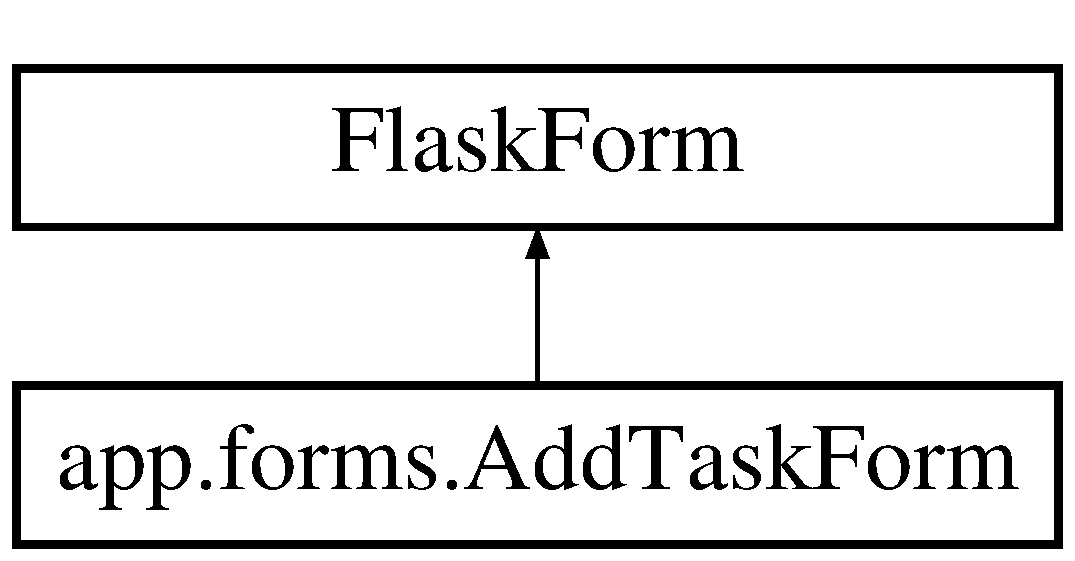
\includegraphics[height=2.000000cm]{classapp_1_1forms_1_1_add_task_form}
\end{center}
\end{figure}
\subsection*{Статические открытые данные}
\begin{DoxyCompactItemize}
\item 
\mbox{\hyperlink{classapp_1_1forms_1_1_add_task_form_a20d3287e025df1bbd1189f5ca5e15d02}{task}} = String\+Field(\textquotesingle{}Задача\textquotesingle{}, validators=\mbox{[}Data\+Required()\mbox{]})
\item 
\mbox{\hyperlink{classapp_1_1forms_1_1_add_task_form_a76e2252402514e3e629b38f0a5bdf37c}{description}} = Text\+Area\+Field(\textquotesingle{}Описание\textquotesingle{}, validators=\mbox{[}Length(min=0, max=128)\mbox{]})
\item 
\mbox{\hyperlink{classapp_1_1forms_1_1_add_task_form_a3ddf0f272307edab62e8855f00a235dc}{submit}} = Submit\+Field(\textquotesingle{}Применить\textquotesingle{})
\end{DoxyCompactItemize}


\subsection{Подробное описание}
Класс формы добавления активности/задачи 


\begin{DoxyParams}{Аргументы}
{\em Flask\+Form} & -\/ родительский класс форм \\
\hline
\end{DoxyParams}


\subsection{Данные класса}
\mbox{\Hypertarget{classapp_1_1forms_1_1_add_task_form_a76e2252402514e3e629b38f0a5bdf37c}\label{classapp_1_1forms_1_1_add_task_form_a76e2252402514e3e629b38f0a5bdf37c}} 
\index{app\+::forms\+::\+Add\+Task\+Form@{app\+::forms\+::\+Add\+Task\+Form}!description@{description}}
\index{description@{description}!app\+::forms\+::\+Add\+Task\+Form@{app\+::forms\+::\+Add\+Task\+Form}}
\subsubsection{\texorpdfstring{description}{description}}
{\footnotesize\ttfamily app.\+forms.\+Add\+Task\+Form.\+description = Text\+Area\+Field(\textquotesingle{}Описание\textquotesingle{}, validators=\mbox{[}Length(min=0, max=128)\mbox{]})\hspace{0.3cm}{\ttfamily [static]}}

\mbox{\Hypertarget{classapp_1_1forms_1_1_add_task_form_a3ddf0f272307edab62e8855f00a235dc}\label{classapp_1_1forms_1_1_add_task_form_a3ddf0f272307edab62e8855f00a235dc}} 
\index{app\+::forms\+::\+Add\+Task\+Form@{app\+::forms\+::\+Add\+Task\+Form}!submit@{submit}}
\index{submit@{submit}!app\+::forms\+::\+Add\+Task\+Form@{app\+::forms\+::\+Add\+Task\+Form}}
\subsubsection{\texorpdfstring{submit}{submit}}
{\footnotesize\ttfamily app.\+forms.\+Add\+Task\+Form.\+submit = Submit\+Field(\textquotesingle{}Применить\textquotesingle{})\hspace{0.3cm}{\ttfamily [static]}}

\mbox{\Hypertarget{classapp_1_1forms_1_1_add_task_form_a20d3287e025df1bbd1189f5ca5e15d02}\label{classapp_1_1forms_1_1_add_task_form_a20d3287e025df1bbd1189f5ca5e15d02}} 
\index{app\+::forms\+::\+Add\+Task\+Form@{app\+::forms\+::\+Add\+Task\+Form}!task@{task}}
\index{task@{task}!app\+::forms\+::\+Add\+Task\+Form@{app\+::forms\+::\+Add\+Task\+Form}}
\subsubsection{\texorpdfstring{task}{task}}
{\footnotesize\ttfamily app.\+forms.\+Add\+Task\+Form.\+task = String\+Field(\textquotesingle{}Задача\textquotesingle{}, validators=\mbox{[}Data\+Required()\mbox{]})\hspace{0.3cm}{\ttfamily [static]}}



Объявления и описания членов класса находятся в файле\+:\begin{DoxyCompactItemize}
\item 
app/\mbox{\hyperlink{forms_8py}{forms.\+py}}\end{DoxyCompactItemize}

\hypertarget{classapp_1_1forms_1_1_edit_profile_form}{}\section{Класс app.\+forms.\+Edit\+Profile\+Form}
\label{classapp_1_1forms_1_1_edit_profile_form}\index{app.\+forms.\+Edit\+Profile\+Form@{app.\+forms.\+Edit\+Profile\+Form}}


Класс формы редактирования профиля  


Граф наследования\+:app.\+forms.\+Edit\+Profile\+Form\+:\begin{figure}[H]
\begin{center}
\leavevmode
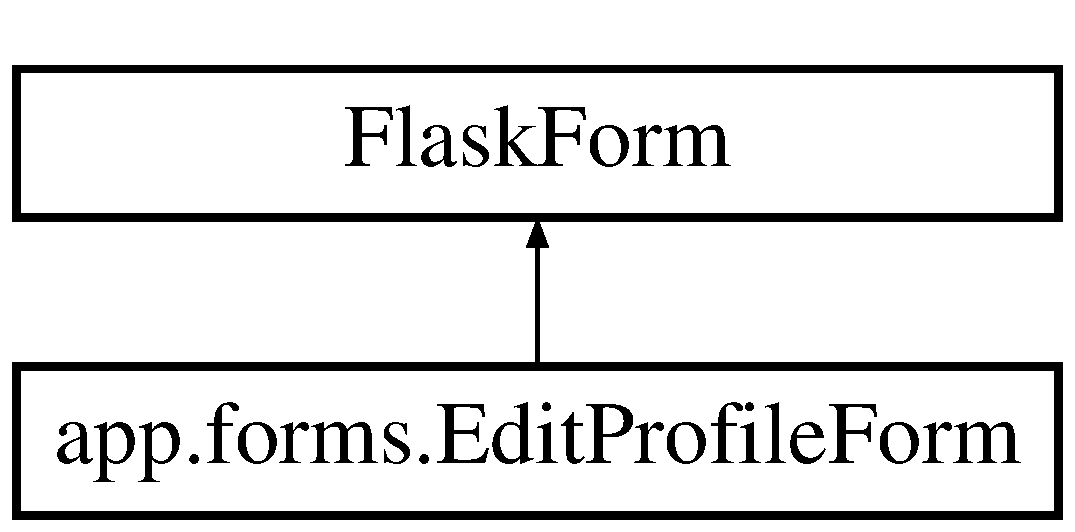
\includegraphics[height=2.000000cm]{classapp_1_1forms_1_1_edit_profile_form}
\end{center}
\end{figure}
\subsection*{Открытые члены}
\begin{DoxyCompactItemize}
\item 
def \mbox{\hyperlink{classapp_1_1forms_1_1_edit_profile_form_ac6fcb8c475148a0190fe489e61e33101}{\+\_\+\+\_\+init\+\_\+\+\_\+}} (self, \mbox{\hyperlink{classapp_1_1forms_1_1_edit_profile_form_a780b5da2adfe5fd308f3e49e83ad343f}{original\+\_\+username}}, args, kwargs)
\begin{DoxyCompactList}\small\item\em Конструктор \end{DoxyCompactList}\item 
def \mbox{\hyperlink{classapp_1_1forms_1_1_edit_profile_form_ae6dab7354d6ef7902de30f80b3fdbdfb}{validate\+\_\+username}} (self, \mbox{\hyperlink{classapp_1_1forms_1_1_edit_profile_form_a57b60e620c9d09de0968b3e456039612}{username}})
\begin{DoxyCompactList}\small\item\em алидация имени пользователя. \end{DoxyCompactList}\end{DoxyCompactItemize}
\subsection*{Открытые атрибуты}
\begin{DoxyCompactItemize}
\item 
\mbox{\hyperlink{classapp_1_1forms_1_1_edit_profile_form_a780b5da2adfe5fd308f3e49e83ad343f}{original\+\_\+username}}
\end{DoxyCompactItemize}
\subsection*{Статические открытые данные}
\begin{DoxyCompactItemize}
\item 
\mbox{\hyperlink{classapp_1_1forms_1_1_edit_profile_form_a57b60e620c9d09de0968b3e456039612}{username}} = String\+Field(\textquotesingle{}Пользователь\textquotesingle{}, validators=\mbox{[}Data\+Required()\mbox{]})
\item 
\mbox{\hyperlink{classapp_1_1forms_1_1_edit_profile_form_ab4d1bb9524c5cbcf8326f4df8888d24f}{about\+\_\+me}} = Text\+Area\+Field(\textquotesingle{}Обо мне\textquotesingle{}, validators=\mbox{[}Length(min=0, max=140)\mbox{]})
\item 
\mbox{\hyperlink{classapp_1_1forms_1_1_edit_profile_form_a75092e1817f3b7a852be060458dc1ba5}{submit}} = Submit\+Field(\textquotesingle{}Применить\textquotesingle{})
\end{DoxyCompactItemize}


\subsection{Подробное описание}
Класс формы редактирования профиля 


\begin{DoxyParams}{Аргументы}
{\em Flask\+Form} & -\/ родительский класс форм \\
\hline
\end{DoxyParams}


\subsection{Конструктор(ы)}
\mbox{\Hypertarget{classapp_1_1forms_1_1_edit_profile_form_ac6fcb8c475148a0190fe489e61e33101}\label{classapp_1_1forms_1_1_edit_profile_form_ac6fcb8c475148a0190fe489e61e33101}} 
\index{app\+::forms\+::\+Edit\+Profile\+Form@{app\+::forms\+::\+Edit\+Profile\+Form}!\+\_\+\+\_\+init\+\_\+\+\_\+@{\+\_\+\+\_\+init\+\_\+\+\_\+}}
\index{\+\_\+\+\_\+init\+\_\+\+\_\+@{\+\_\+\+\_\+init\+\_\+\+\_\+}!app\+::forms\+::\+Edit\+Profile\+Form@{app\+::forms\+::\+Edit\+Profile\+Form}}
\subsubsection{\texorpdfstring{\+\_\+\+\_\+init\+\_\+\+\_\+()}{\_\_init\_\_()}}
{\footnotesize\ttfamily def app.\+forms.\+Edit\+Profile\+Form.\+\_\+\+\_\+init\+\_\+\+\_\+ (\begin{DoxyParamCaption}\item[{}]{self,  }\item[{}]{original\+\_\+username,  }\item[{}]{args,  }\item[{}]{kwargs }\end{DoxyParamCaption})}



Конструктор 


\begin{DoxyParams}{Аргументы}
{\em original\+\_\+username} & -\/ имя пользователя. \\
\hline
\end{DoxyParams}


\subsection{Методы}
\mbox{\Hypertarget{classapp_1_1forms_1_1_edit_profile_form_ae6dab7354d6ef7902de30f80b3fdbdfb}\label{classapp_1_1forms_1_1_edit_profile_form_ae6dab7354d6ef7902de30f80b3fdbdfb}} 
\index{app\+::forms\+::\+Edit\+Profile\+Form@{app\+::forms\+::\+Edit\+Profile\+Form}!validate\+\_\+username@{validate\+\_\+username}}
\index{validate\+\_\+username@{validate\+\_\+username}!app\+::forms\+::\+Edit\+Profile\+Form@{app\+::forms\+::\+Edit\+Profile\+Form}}
\subsubsection{\texorpdfstring{validate\+\_\+username()}{validate\_username()}}
{\footnotesize\ttfamily def app.\+forms.\+Edit\+Profile\+Form.\+validate\+\_\+username (\begin{DoxyParamCaption}\item[{}]{self,  }\item[{}]{username }\end{DoxyParamCaption})}



алидация имени пользователя. 


\begin{DoxyParams}{Аргументы}
{\em username} & -\/ имя пользователя \\
\hline
\end{DoxyParams}


\subsection{Данные класса}
\mbox{\Hypertarget{classapp_1_1forms_1_1_edit_profile_form_ab4d1bb9524c5cbcf8326f4df8888d24f}\label{classapp_1_1forms_1_1_edit_profile_form_ab4d1bb9524c5cbcf8326f4df8888d24f}} 
\index{app\+::forms\+::\+Edit\+Profile\+Form@{app\+::forms\+::\+Edit\+Profile\+Form}!about\+\_\+me@{about\+\_\+me}}
\index{about\+\_\+me@{about\+\_\+me}!app\+::forms\+::\+Edit\+Profile\+Form@{app\+::forms\+::\+Edit\+Profile\+Form}}
\subsubsection{\texorpdfstring{about\+\_\+me}{about\_me}}
{\footnotesize\ttfamily app.\+forms.\+Edit\+Profile\+Form.\+about\+\_\+me = Text\+Area\+Field(\textquotesingle{}Обо мне\textquotesingle{}, validators=\mbox{[}Length(min=0, max=140)\mbox{]})\hspace{0.3cm}{\ttfamily [static]}}

\mbox{\Hypertarget{classapp_1_1forms_1_1_edit_profile_form_a780b5da2adfe5fd308f3e49e83ad343f}\label{classapp_1_1forms_1_1_edit_profile_form_a780b5da2adfe5fd308f3e49e83ad343f}} 
\index{app\+::forms\+::\+Edit\+Profile\+Form@{app\+::forms\+::\+Edit\+Profile\+Form}!original\+\_\+username@{original\+\_\+username}}
\index{original\+\_\+username@{original\+\_\+username}!app\+::forms\+::\+Edit\+Profile\+Form@{app\+::forms\+::\+Edit\+Profile\+Form}}
\subsubsection{\texorpdfstring{original\+\_\+username}{original\_username}}
{\footnotesize\ttfamily app.\+forms.\+Edit\+Profile\+Form.\+original\+\_\+username}

\mbox{\Hypertarget{classapp_1_1forms_1_1_edit_profile_form_a75092e1817f3b7a852be060458dc1ba5}\label{classapp_1_1forms_1_1_edit_profile_form_a75092e1817f3b7a852be060458dc1ba5}} 
\index{app\+::forms\+::\+Edit\+Profile\+Form@{app\+::forms\+::\+Edit\+Profile\+Form}!submit@{submit}}
\index{submit@{submit}!app\+::forms\+::\+Edit\+Profile\+Form@{app\+::forms\+::\+Edit\+Profile\+Form}}
\subsubsection{\texorpdfstring{submit}{submit}}
{\footnotesize\ttfamily app.\+forms.\+Edit\+Profile\+Form.\+submit = Submit\+Field(\textquotesingle{}Применить\textquotesingle{})\hspace{0.3cm}{\ttfamily [static]}}

\mbox{\Hypertarget{classapp_1_1forms_1_1_edit_profile_form_a57b60e620c9d09de0968b3e456039612}\label{classapp_1_1forms_1_1_edit_profile_form_a57b60e620c9d09de0968b3e456039612}} 
\index{app\+::forms\+::\+Edit\+Profile\+Form@{app\+::forms\+::\+Edit\+Profile\+Form}!username@{username}}
\index{username@{username}!app\+::forms\+::\+Edit\+Profile\+Form@{app\+::forms\+::\+Edit\+Profile\+Form}}
\subsubsection{\texorpdfstring{username}{username}}
{\footnotesize\ttfamily app.\+forms.\+Edit\+Profile\+Form.\+username = String\+Field(\textquotesingle{}Пользователь\textquotesingle{}, validators=\mbox{[}Data\+Required()\mbox{]})\hspace{0.3cm}{\ttfamily [static]}}



Объявления и описания членов класса находятся в файле\+:\begin{DoxyCompactItemize}
\item 
app/\mbox{\hyperlink{forms_8py}{forms.\+py}}\end{DoxyCompactItemize}

\hypertarget{classapp_1_1forms_1_1_login_form}{}\section{Класс app.\+forms.\+Login\+Form}
\label{classapp_1_1forms_1_1_login_form}\index{app.\+forms.\+Login\+Form@{app.\+forms.\+Login\+Form}}


Класс формы входа  


Граф наследования\+:app.\+forms.\+Login\+Form\+:\begin{figure}[H]
\begin{center}
\leavevmode
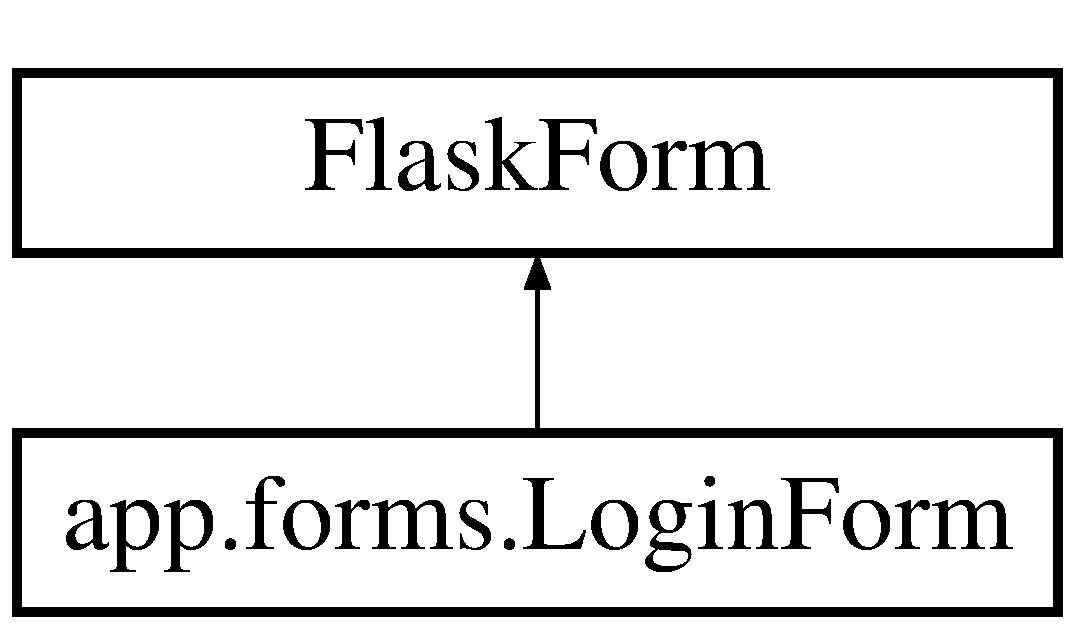
\includegraphics[height=2.000000cm]{classapp_1_1forms_1_1_login_form}
\end{center}
\end{figure}
\subsection*{Статические открытые данные}
\begin{DoxyCompactItemize}
\item 
\mbox{\hyperlink{classapp_1_1forms_1_1_login_form_acc32a2914184aa30d464bf3ae29d3fe8}{username}} = String\+Field(\textquotesingle{}Пользователь\textquotesingle{}, validators=\mbox{[}Data\+Required()\mbox{]})
\item 
\mbox{\hyperlink{classapp_1_1forms_1_1_login_form_a53abb2f26f647359d44d7ef5fc2756d7}{password}} = Password\+Field(\textquotesingle{}Пароль\textquotesingle{}, validators=\mbox{[}Data\+Required()\mbox{]})
\item 
\mbox{\hyperlink{classapp_1_1forms_1_1_login_form_ad2b8871e15dc50fc2d21fc937a2dc2f1}{remember\+\_\+me}} = Boolean\+Field(\textquotesingle{}Запомнить\textquotesingle{})
\item 
\mbox{\hyperlink{classapp_1_1forms_1_1_login_form_aeedc9621e8588a0fd186fefc813f2bda}{submit}} = Submit\+Field(\textquotesingle{}Войти\textquotesingle{})
\end{DoxyCompactItemize}


\subsection{Подробное описание}
Класс формы входа 


\begin{DoxyParams}{Аргументы}
{\em Flask\+Form} & -\/ родительский класс форм \\
\hline
\end{DoxyParams}


\subsection{Данные класса}
\mbox{\Hypertarget{classapp_1_1forms_1_1_login_form_a53abb2f26f647359d44d7ef5fc2756d7}\label{classapp_1_1forms_1_1_login_form_a53abb2f26f647359d44d7ef5fc2756d7}} 
\index{app\+::forms\+::\+Login\+Form@{app\+::forms\+::\+Login\+Form}!password@{password}}
\index{password@{password}!app\+::forms\+::\+Login\+Form@{app\+::forms\+::\+Login\+Form}}
\subsubsection{\texorpdfstring{password}{password}}
{\footnotesize\ttfamily app.\+forms.\+Login\+Form.\+password = Password\+Field(\textquotesingle{}Пароль\textquotesingle{}, validators=\mbox{[}Data\+Required()\mbox{]})\hspace{0.3cm}{\ttfamily [static]}}

\mbox{\Hypertarget{classapp_1_1forms_1_1_login_form_ad2b8871e15dc50fc2d21fc937a2dc2f1}\label{classapp_1_1forms_1_1_login_form_ad2b8871e15dc50fc2d21fc937a2dc2f1}} 
\index{app\+::forms\+::\+Login\+Form@{app\+::forms\+::\+Login\+Form}!remember\+\_\+me@{remember\+\_\+me}}
\index{remember\+\_\+me@{remember\+\_\+me}!app\+::forms\+::\+Login\+Form@{app\+::forms\+::\+Login\+Form}}
\subsubsection{\texorpdfstring{remember\+\_\+me}{remember\_me}}
{\footnotesize\ttfamily app.\+forms.\+Login\+Form.\+remember\+\_\+me = Boolean\+Field(\textquotesingle{}Запомнить\textquotesingle{})\hspace{0.3cm}{\ttfamily [static]}}

\mbox{\Hypertarget{classapp_1_1forms_1_1_login_form_aeedc9621e8588a0fd186fefc813f2bda}\label{classapp_1_1forms_1_1_login_form_aeedc9621e8588a0fd186fefc813f2bda}} 
\index{app\+::forms\+::\+Login\+Form@{app\+::forms\+::\+Login\+Form}!submit@{submit}}
\index{submit@{submit}!app\+::forms\+::\+Login\+Form@{app\+::forms\+::\+Login\+Form}}
\subsubsection{\texorpdfstring{submit}{submit}}
{\footnotesize\ttfamily app.\+forms.\+Login\+Form.\+submit = Submit\+Field(\textquotesingle{}Войти\textquotesingle{})\hspace{0.3cm}{\ttfamily [static]}}

\mbox{\Hypertarget{classapp_1_1forms_1_1_login_form_acc32a2914184aa30d464bf3ae29d3fe8}\label{classapp_1_1forms_1_1_login_form_acc32a2914184aa30d464bf3ae29d3fe8}} 
\index{app\+::forms\+::\+Login\+Form@{app\+::forms\+::\+Login\+Form}!username@{username}}
\index{username@{username}!app\+::forms\+::\+Login\+Form@{app\+::forms\+::\+Login\+Form}}
\subsubsection{\texorpdfstring{username}{username}}
{\footnotesize\ttfamily app.\+forms.\+Login\+Form.\+username = String\+Field(\textquotesingle{}Пользователь\textquotesingle{}, validators=\mbox{[}Data\+Required()\mbox{]})\hspace{0.3cm}{\ttfamily [static]}}



Объявления и описания членов класса находятся в файле\+:\begin{DoxyCompactItemize}
\item 
app/\mbox{\hyperlink{forms_8py}{forms.\+py}}\end{DoxyCompactItemize}

\hypertarget{classapp_1_1forms_1_1_registration_form}{}\section{Класс app.\+forms.\+Registration\+Form}
\label{classapp_1_1forms_1_1_registration_form}\index{app.\+forms.\+Registration\+Form@{app.\+forms.\+Registration\+Form}}


Класс формы регистрации  


Граф наследования\+:app.\+forms.\+Registration\+Form\+:\begin{figure}[H]
\begin{center}
\leavevmode
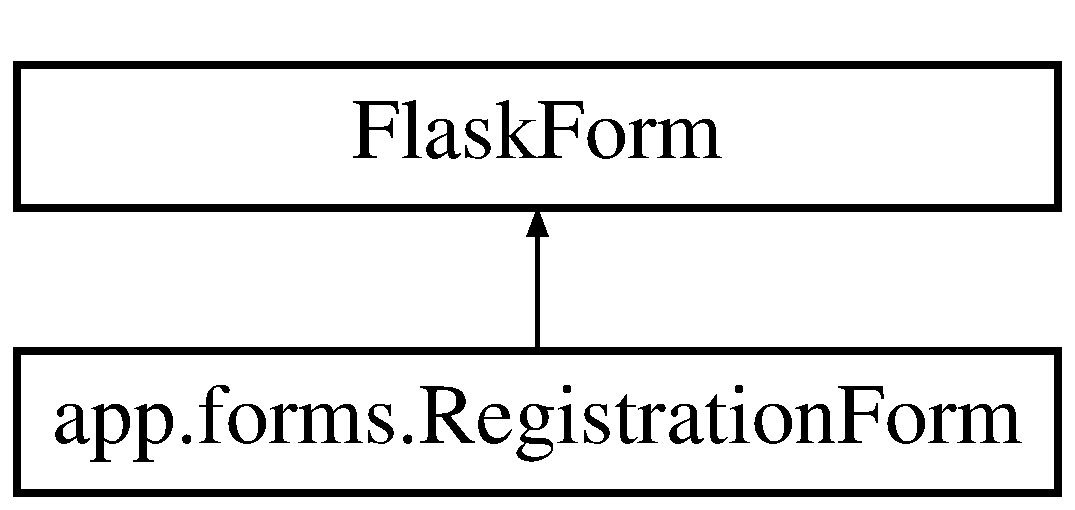
\includegraphics[height=2.000000cm]{classapp_1_1forms_1_1_registration_form}
\end{center}
\end{figure}
\subsection*{Открытые члены}
\begin{DoxyCompactItemize}
\item 
def \mbox{\hyperlink{classapp_1_1forms_1_1_registration_form_a69ecc2875e684131ba0eeb9451e9c47c}{validate\+\_\+username}} (self, \mbox{\hyperlink{classapp_1_1forms_1_1_registration_form_ac4f31c06a04cfadf0ecf269bcb65c29b}{username}})
\begin{DoxyCompactList}\small\item\em Валидация имени пользователя. \end{DoxyCompactList}\item 
def \mbox{\hyperlink{classapp_1_1forms_1_1_registration_form_a03ad81c1e7ea6eaad93fb503be3f6f4b}{validate\+\_\+email}} (self, \mbox{\hyperlink{classapp_1_1forms_1_1_registration_form_af98d363c036c4b9afcf8ac4bc2d3ee6a}{email}})
\begin{DoxyCompactList}\small\item\em Валидация адреса e-\/mail. \end{DoxyCompactList}\end{DoxyCompactItemize}
\subsection*{Статические открытые данные}
\begin{DoxyCompactItemize}
\item 
\mbox{\hyperlink{classapp_1_1forms_1_1_registration_form_ac4f31c06a04cfadf0ecf269bcb65c29b}{username}} = String\+Field(\textquotesingle{}Пользователь\textquotesingle{}, validators=\mbox{[}Data\+Required()\mbox{]})
\item 
\mbox{\hyperlink{classapp_1_1forms_1_1_registration_form_af98d363c036c4b9afcf8ac4bc2d3ee6a}{email}} = String\+Field(\textquotesingle{}Email\textquotesingle{}, validators=\mbox{[}Data\+Required(), Email()\mbox{]})
\item 
\mbox{\hyperlink{classapp_1_1forms_1_1_registration_form_a20158cd008a957749d4315a3acbdc114}{password}} = Password\+Field(\textquotesingle{}Пароль\textquotesingle{}, validators=\mbox{[}Data\+Required()\mbox{]})
\item 
\mbox{\hyperlink{classapp_1_1forms_1_1_registration_form_a29d1668141132f75f709ae0d02ae4a2c}{password2}}
\item 
\mbox{\hyperlink{classapp_1_1forms_1_1_registration_form_a64e8b7e4c4567cdd41fb495c8473748a}{submit}} = Submit\+Field(\textquotesingle{}Зарегистрироваться\textquotesingle{})
\end{DoxyCompactItemize}


\subsection{Подробное описание}
Класс формы регистрации 


\begin{DoxyParams}{Аргументы}
{\em Flask\+Form} & -\/ родительский класс форм \\
\hline
\end{DoxyParams}


\subsection{Методы}
\mbox{\Hypertarget{classapp_1_1forms_1_1_registration_form_a03ad81c1e7ea6eaad93fb503be3f6f4b}\label{classapp_1_1forms_1_1_registration_form_a03ad81c1e7ea6eaad93fb503be3f6f4b}} 
\index{app\+::forms\+::\+Registration\+Form@{app\+::forms\+::\+Registration\+Form}!validate\+\_\+email@{validate\+\_\+email}}
\index{validate\+\_\+email@{validate\+\_\+email}!app\+::forms\+::\+Registration\+Form@{app\+::forms\+::\+Registration\+Form}}
\subsubsection{\texorpdfstring{validate\+\_\+email()}{validate\_email()}}
{\footnotesize\ttfamily def app.\+forms.\+Registration\+Form.\+validate\+\_\+email (\begin{DoxyParamCaption}\item[{}]{self,  }\item[{}]{email }\end{DoxyParamCaption})}



Валидация адреса e-\/mail. 


\begin{DoxyParams}{Аргументы}
{\em email} & -\/ электронная почта \\
\hline
\end{DoxyParams}
\mbox{\Hypertarget{classapp_1_1forms_1_1_registration_form_a69ecc2875e684131ba0eeb9451e9c47c}\label{classapp_1_1forms_1_1_registration_form_a69ecc2875e684131ba0eeb9451e9c47c}} 
\index{app\+::forms\+::\+Registration\+Form@{app\+::forms\+::\+Registration\+Form}!validate\+\_\+username@{validate\+\_\+username}}
\index{validate\+\_\+username@{validate\+\_\+username}!app\+::forms\+::\+Registration\+Form@{app\+::forms\+::\+Registration\+Form}}
\subsubsection{\texorpdfstring{validate\+\_\+username()}{validate\_username()}}
{\footnotesize\ttfamily def app.\+forms.\+Registration\+Form.\+validate\+\_\+username (\begin{DoxyParamCaption}\item[{}]{self,  }\item[{}]{username }\end{DoxyParamCaption})}



Валидация имени пользователя. 


\begin{DoxyParams}{Аргументы}
{\em username} & -\/ имя пользователя \\
\hline
\end{DoxyParams}


\subsection{Данные класса}
\mbox{\Hypertarget{classapp_1_1forms_1_1_registration_form_af98d363c036c4b9afcf8ac4bc2d3ee6a}\label{classapp_1_1forms_1_1_registration_form_af98d363c036c4b9afcf8ac4bc2d3ee6a}} 
\index{app\+::forms\+::\+Registration\+Form@{app\+::forms\+::\+Registration\+Form}!email@{email}}
\index{email@{email}!app\+::forms\+::\+Registration\+Form@{app\+::forms\+::\+Registration\+Form}}
\subsubsection{\texorpdfstring{email}{email}}
{\footnotesize\ttfamily app.\+forms.\+Registration\+Form.\+email = String\+Field(\textquotesingle{}Email\textquotesingle{}, validators=\mbox{[}Data\+Required(), Email()\mbox{]})\hspace{0.3cm}{\ttfamily [static]}}

\mbox{\Hypertarget{classapp_1_1forms_1_1_registration_form_a20158cd008a957749d4315a3acbdc114}\label{classapp_1_1forms_1_1_registration_form_a20158cd008a957749d4315a3acbdc114}} 
\index{app\+::forms\+::\+Registration\+Form@{app\+::forms\+::\+Registration\+Form}!password@{password}}
\index{password@{password}!app\+::forms\+::\+Registration\+Form@{app\+::forms\+::\+Registration\+Form}}
\subsubsection{\texorpdfstring{password}{password}}
{\footnotesize\ttfamily app.\+forms.\+Registration\+Form.\+password = Password\+Field(\textquotesingle{}Пароль\textquotesingle{}, validators=\mbox{[}Data\+Required()\mbox{]})\hspace{0.3cm}{\ttfamily [static]}}

\mbox{\Hypertarget{classapp_1_1forms_1_1_registration_form_a29d1668141132f75f709ae0d02ae4a2c}\label{classapp_1_1forms_1_1_registration_form_a29d1668141132f75f709ae0d02ae4a2c}} 
\index{app\+::forms\+::\+Registration\+Form@{app\+::forms\+::\+Registration\+Form}!password2@{password2}}
\index{password2@{password2}!app\+::forms\+::\+Registration\+Form@{app\+::forms\+::\+Registration\+Form}}
\subsubsection{\texorpdfstring{password2}{password2}}
{\footnotesize\ttfamily app.\+forms.\+Registration\+Form.\+password2\hspace{0.3cm}{\ttfamily [static]}}

{\bfseries Инициализатор}
\begin{DoxyCode}
=  PasswordField(
        \textcolor{stringliteral}{'Повторите пароль'}, validators=[DataRequired(), EqualTo(\textcolor{stringliteral}{'password'})])
\end{DoxyCode}
\mbox{\Hypertarget{classapp_1_1forms_1_1_registration_form_a64e8b7e4c4567cdd41fb495c8473748a}\label{classapp_1_1forms_1_1_registration_form_a64e8b7e4c4567cdd41fb495c8473748a}} 
\index{app\+::forms\+::\+Registration\+Form@{app\+::forms\+::\+Registration\+Form}!submit@{submit}}
\index{submit@{submit}!app\+::forms\+::\+Registration\+Form@{app\+::forms\+::\+Registration\+Form}}
\subsubsection{\texorpdfstring{submit}{submit}}
{\footnotesize\ttfamily app.\+forms.\+Registration\+Form.\+submit = Submit\+Field(\textquotesingle{}Зарегистрироваться\textquotesingle{})\hspace{0.3cm}{\ttfamily [static]}}

\mbox{\Hypertarget{classapp_1_1forms_1_1_registration_form_ac4f31c06a04cfadf0ecf269bcb65c29b}\label{classapp_1_1forms_1_1_registration_form_ac4f31c06a04cfadf0ecf269bcb65c29b}} 
\index{app\+::forms\+::\+Registration\+Form@{app\+::forms\+::\+Registration\+Form}!username@{username}}
\index{username@{username}!app\+::forms\+::\+Registration\+Form@{app\+::forms\+::\+Registration\+Form}}
\subsubsection{\texorpdfstring{username}{username}}
{\footnotesize\ttfamily app.\+forms.\+Registration\+Form.\+username = String\+Field(\textquotesingle{}Пользователь\textquotesingle{}, validators=\mbox{[}Data\+Required()\mbox{]})\hspace{0.3cm}{\ttfamily [static]}}



Объявления и описания членов класса находятся в файле\+:\begin{DoxyCompactItemize}
\item 
app/\mbox{\hyperlink{forms_8py}{forms.\+py}}\end{DoxyCompactItemize}

\hypertarget{classapp_1_1models_1_1_task}{}\section{Класс app.\+models.\+Task}
\label{classapp_1_1models_1_1_task}\index{app.\+models.\+Task@{app.\+models.\+Task}}


Класс активностей  


Граф наследования\+:app.\+models.\+Task\+:\begin{figure}[H]
\begin{center}
\leavevmode
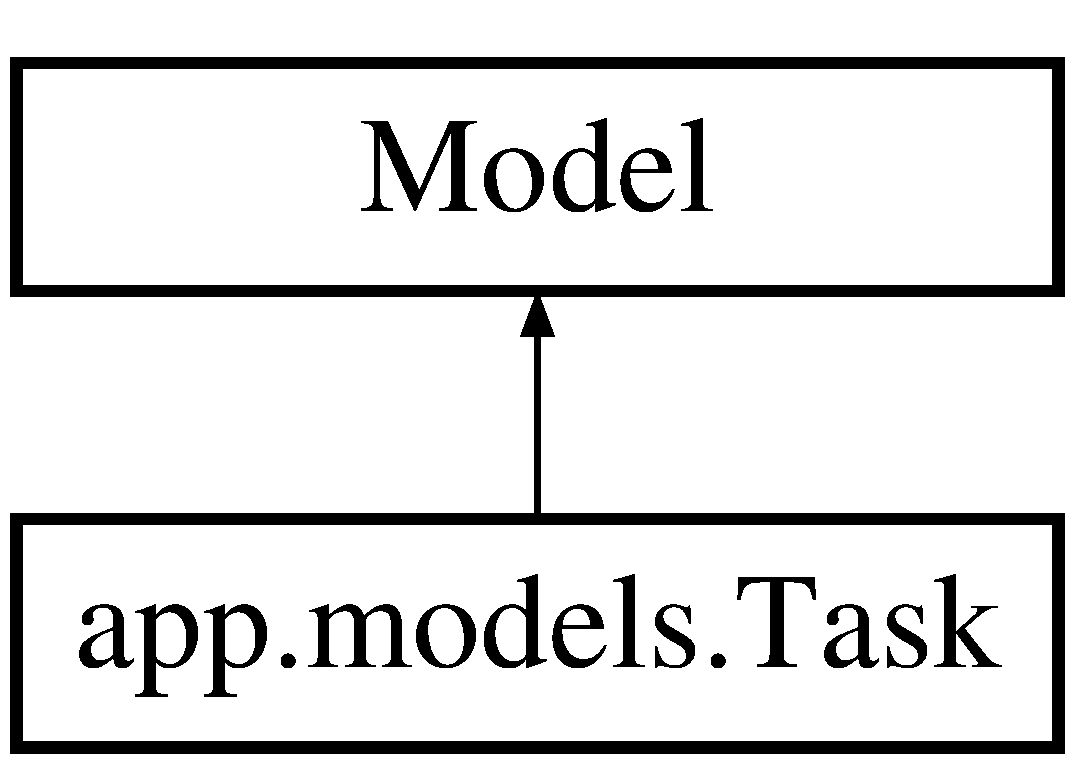
\includegraphics[height=2.000000cm]{classapp_1_1models_1_1_task}
\end{center}
\end{figure}
\subsection*{Открытые члены}
\begin{DoxyCompactItemize}
\item 
def \mbox{\hyperlink{classapp_1_1models_1_1_task_a878962473a5595e85e499f7572bd9ebd}{\+\_\+\+\_\+repr\+\_\+\+\_\+}} (self)
\begin{DoxyCompactList}\small\item\em Представление объекта \mbox{\hyperlink{classapp_1_1models_1_1_task}{Task}} при печати. \end{DoxyCompactList}\end{DoxyCompactItemize}
\subsection*{Статические открытые данные}
\begin{DoxyCompactItemize}
\item 
\mbox{\hyperlink{classapp_1_1models_1_1_task_aad4ef074a554fa0ffe977cd4b934275a}{id}} = db.\+Column(db.\+Integer, primary\+\_\+key=True)
\item 
\mbox{\hyperlink{classapp_1_1models_1_1_task_aeab47ec2eef251bb3cb1b34f7ae140df}{task}} = db.\+Column(db.\+String(64), unique=True)
\item 
\mbox{\hyperlink{classapp_1_1models_1_1_task_af0ef177b07b0af27261c072ed5e550ee}{description}} = db.\+Column(db.\+String(128))
\item 
\mbox{\hyperlink{classapp_1_1models_1_1_task_aca1ae8c419c42f9122c02d0c788672cd}{start}} = db.\+Column(db.\+Date\+Time, index=True)
\item 
\mbox{\hyperlink{classapp_1_1models_1_1_task_a5fd4eea12e4fd7a4db19f3a04bf2a32f}{stop}} = db.\+Column(db.\+Date\+Time, index=True)
\item 
\mbox{\hyperlink{classapp_1_1models_1_1_task_a72b3ad4ca2c7c9d47262523bc91526ae}{user\+\_\+id}} = db.\+Column(db.\+Integer, db.\+Foreign\+Key(\textquotesingle{}user.\+id\textquotesingle{}))
\end{DoxyCompactItemize}


\subsection{Подробное описание}
Класс активностей 


\begin{DoxyParams}{Аргументы}
{\em db.\+Model} & -\/ класс моделей S\+Q\+L\+Alchemy \\
\hline
\end{DoxyParams}


\subsection{Методы}
\mbox{\Hypertarget{classapp_1_1models_1_1_task_a878962473a5595e85e499f7572bd9ebd}\label{classapp_1_1models_1_1_task_a878962473a5595e85e499f7572bd9ebd}} 
\index{app\+::models\+::\+Task@{app\+::models\+::\+Task}!\+\_\+\+\_\+repr\+\_\+\+\_\+@{\+\_\+\+\_\+repr\+\_\+\+\_\+}}
\index{\+\_\+\+\_\+repr\+\_\+\+\_\+@{\+\_\+\+\_\+repr\+\_\+\+\_\+}!app\+::models\+::\+Task@{app\+::models\+::\+Task}}
\subsubsection{\texorpdfstring{\+\_\+\+\_\+repr\+\_\+\+\_\+()}{\_\_repr\_\_()}}
{\footnotesize\ttfamily def app.\+models.\+Task.\+\_\+\+\_\+repr\+\_\+\+\_\+ (\begin{DoxyParamCaption}\item[{}]{self }\end{DoxyParamCaption})}



Представление объекта \mbox{\hyperlink{classapp_1_1models_1_1_task}{Task}} при печати. 



\subsection{Данные класса}
\mbox{\Hypertarget{classapp_1_1models_1_1_task_af0ef177b07b0af27261c072ed5e550ee}\label{classapp_1_1models_1_1_task_af0ef177b07b0af27261c072ed5e550ee}} 
\index{app\+::models\+::\+Task@{app\+::models\+::\+Task}!description@{description}}
\index{description@{description}!app\+::models\+::\+Task@{app\+::models\+::\+Task}}
\subsubsection{\texorpdfstring{description}{description}}
{\footnotesize\ttfamily app.\+models.\+Task.\+description = db.\+Column(db.\+String(128))\hspace{0.3cm}{\ttfamily [static]}}

\mbox{\Hypertarget{classapp_1_1models_1_1_task_aad4ef074a554fa0ffe977cd4b934275a}\label{classapp_1_1models_1_1_task_aad4ef074a554fa0ffe977cd4b934275a}} 
\index{app\+::models\+::\+Task@{app\+::models\+::\+Task}!id@{id}}
\index{id@{id}!app\+::models\+::\+Task@{app\+::models\+::\+Task}}
\subsubsection{\texorpdfstring{id}{id}}
{\footnotesize\ttfamily app.\+models.\+Task.\+id = db.\+Column(db.\+Integer, primary\+\_\+key=True)\hspace{0.3cm}{\ttfamily [static]}}

\mbox{\Hypertarget{classapp_1_1models_1_1_task_aca1ae8c419c42f9122c02d0c788672cd}\label{classapp_1_1models_1_1_task_aca1ae8c419c42f9122c02d0c788672cd}} 
\index{app\+::models\+::\+Task@{app\+::models\+::\+Task}!start@{start}}
\index{start@{start}!app\+::models\+::\+Task@{app\+::models\+::\+Task}}
\subsubsection{\texorpdfstring{start}{start}}
{\footnotesize\ttfamily app.\+models.\+Task.\+start = db.\+Column(db.\+Date\+Time, index=True)\hspace{0.3cm}{\ttfamily [static]}}

\mbox{\Hypertarget{classapp_1_1models_1_1_task_a5fd4eea12e4fd7a4db19f3a04bf2a32f}\label{classapp_1_1models_1_1_task_a5fd4eea12e4fd7a4db19f3a04bf2a32f}} 
\index{app\+::models\+::\+Task@{app\+::models\+::\+Task}!stop@{stop}}
\index{stop@{stop}!app\+::models\+::\+Task@{app\+::models\+::\+Task}}
\subsubsection{\texorpdfstring{stop}{stop}}
{\footnotesize\ttfamily app.\+models.\+Task.\+stop = db.\+Column(db.\+Date\+Time, index=True)\hspace{0.3cm}{\ttfamily [static]}}

\mbox{\Hypertarget{classapp_1_1models_1_1_task_aeab47ec2eef251bb3cb1b34f7ae140df}\label{classapp_1_1models_1_1_task_aeab47ec2eef251bb3cb1b34f7ae140df}} 
\index{app\+::models\+::\+Task@{app\+::models\+::\+Task}!task@{task}}
\index{task@{task}!app\+::models\+::\+Task@{app\+::models\+::\+Task}}
\subsubsection{\texorpdfstring{task}{task}}
{\footnotesize\ttfamily app.\+models.\+Task.\+task = db.\+Column(db.\+String(64), unique=True)\hspace{0.3cm}{\ttfamily [static]}}

\mbox{\Hypertarget{classapp_1_1models_1_1_task_a72b3ad4ca2c7c9d47262523bc91526ae}\label{classapp_1_1models_1_1_task_a72b3ad4ca2c7c9d47262523bc91526ae}} 
\index{app\+::models\+::\+Task@{app\+::models\+::\+Task}!user\+\_\+id@{user\+\_\+id}}
\index{user\+\_\+id@{user\+\_\+id}!app\+::models\+::\+Task@{app\+::models\+::\+Task}}
\subsubsection{\texorpdfstring{user\+\_\+id}{user\_id}}
{\footnotesize\ttfamily app.\+models.\+Task.\+user\+\_\+id = db.\+Column(db.\+Integer, db.\+Foreign\+Key(\textquotesingle{}user.\+id\textquotesingle{}))\hspace{0.3cm}{\ttfamily [static]}}



Объявления и описания членов класса находятся в файле\+:\begin{DoxyCompactItemize}
\item 
app/\mbox{\hyperlink{models_8py}{models.\+py}}\end{DoxyCompactItemize}

\hypertarget{classapp_1_1models_1_1_user}{}\section{Класс app.\+models.\+User}
\label{classapp_1_1models_1_1_user}\index{app.\+models.\+User@{app.\+models.\+User}}


Класс пользователей  


Граф наследования\+:app.\+models.\+User\+:\begin{figure}[H]
\begin{center}
\leavevmode
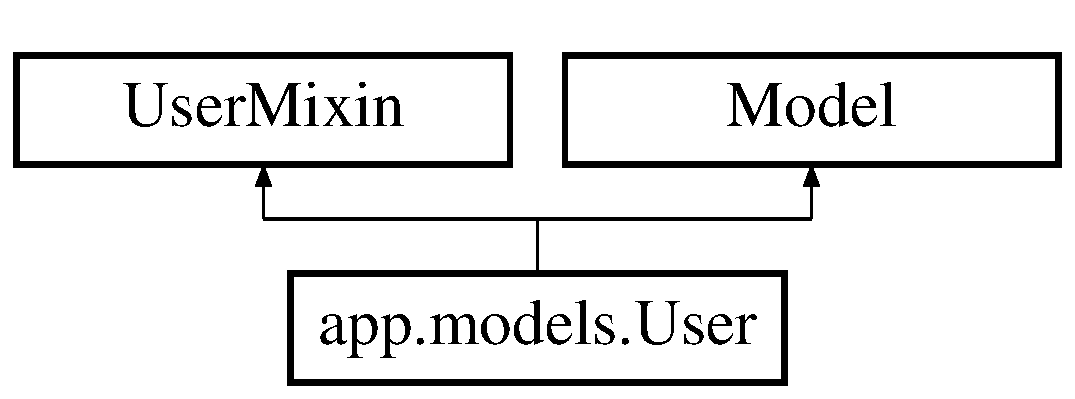
\includegraphics[height=2.000000cm]{classapp_1_1models_1_1_user}
\end{center}
\end{figure}
\subsection*{Открытые члены}
\begin{DoxyCompactItemize}
\item 
def \mbox{\hyperlink{classapp_1_1models_1_1_user_a7569b5686d9aa38eb081b4d811338d9f}{\+\_\+\+\_\+repr\+\_\+\+\_\+}} (self)
\begin{DoxyCompactList}\small\item\em Представление объекта \mbox{\hyperlink{classapp_1_1models_1_1_user}{User}} при печати. \end{DoxyCompactList}\item 
def \mbox{\hyperlink{classapp_1_1models_1_1_user_aa8be40797a363177fd35d541da309297}{set\+\_\+password}} (self, password)
\begin{DoxyCompactList}\small\item\em Установка пароля. \end{DoxyCompactList}\item 
def \mbox{\hyperlink{classapp_1_1models_1_1_user_ab75430896da76337b5eb18763f2a18c3}{check\+\_\+password}} (self, password)
\begin{DoxyCompactList}\small\item\em Проверка пароля \end{DoxyCompactList}\item 
def \mbox{\hyperlink{classapp_1_1models_1_1_user_afbfdcc8d14cb2c09cca368406be71764}{avatar}} (self, size)
\begin{DoxyCompactList}\small\item\em Установка аватара. \end{DoxyCompactList}\end{DoxyCompactItemize}
\subsection*{Статические открытые данные}
\begin{DoxyCompactItemize}
\item 
\mbox{\hyperlink{classapp_1_1models_1_1_user_ad28c4b49ed1a0a093e086410d9da2df2}{id}} = db.\+Column(db.\+Integer, primary\+\_\+key=True)
\item 
\mbox{\hyperlink{classapp_1_1models_1_1_user_aec05013ad6d15a43fcd996241fc32912}{username}} = db.\+Column(db.\+String(64), index=True, unique=True)
\item 
\mbox{\hyperlink{classapp_1_1models_1_1_user_abede62bbd3c533d9532f44a7181bb970}{email}} = db.\+Column(db.\+String(120), index=True, unique=True)
\item 
\mbox{\hyperlink{classapp_1_1models_1_1_user_a80ee86a4974fc0e6ae597288d2e2fe43}{password\+\_\+hash}} = db.\+Column(db.\+String(128))
\item 
\mbox{\hyperlink{classapp_1_1models_1_1_user_a9d486736caa6cb4e1878bf6ec022ba36}{tasks}} = db.\+relationship(\textquotesingle{}\mbox{\hyperlink{classapp_1_1models_1_1_task}{Task}}\textquotesingle{}, backref=\textquotesingle{}author\textquotesingle{}, lazy=\textquotesingle{}dynamic\textquotesingle{})
\item 
\mbox{\hyperlink{classapp_1_1models_1_1_user_ae73eebfaf616e6c86471d14b89f18a85}{about\+\_\+me}} = db.\+Column(db.\+String(140))
\item 
\mbox{\hyperlink{classapp_1_1models_1_1_user_a9b0d23d616421ef30c01e87bb92f6aea}{last\+\_\+seen}} = db.\+Column(db.\+Date\+Time, default=datetime.\+utcnow)
\end{DoxyCompactItemize}


\subsection{Подробное описание}
Класс пользователей 


\begin{DoxyParams}{Аргументы}
{\em User\+Mixin} & -\/ класс, который включает в себя общие реализации классов пользовательских моделей \\
\hline
{\em db.\+Model} & -\/ класс моделей S\+Q\+L\+Alchemy \\
\hline
\end{DoxyParams}


\subsection{Методы}
\mbox{\Hypertarget{classapp_1_1models_1_1_user_a7569b5686d9aa38eb081b4d811338d9f}\label{classapp_1_1models_1_1_user_a7569b5686d9aa38eb081b4d811338d9f}} 
\index{app\+::models\+::\+User@{app\+::models\+::\+User}!\+\_\+\+\_\+repr\+\_\+\+\_\+@{\+\_\+\+\_\+repr\+\_\+\+\_\+}}
\index{\+\_\+\+\_\+repr\+\_\+\+\_\+@{\+\_\+\+\_\+repr\+\_\+\+\_\+}!app\+::models\+::\+User@{app\+::models\+::\+User}}
\subsubsection{\texorpdfstring{\+\_\+\+\_\+repr\+\_\+\+\_\+()}{\_\_repr\_\_()}}
{\footnotesize\ttfamily def app.\+models.\+User.\+\_\+\+\_\+repr\+\_\+\+\_\+ (\begin{DoxyParamCaption}\item[{}]{self }\end{DoxyParamCaption})}



Представление объекта \mbox{\hyperlink{classapp_1_1models_1_1_user}{User}} при печати. 

\mbox{\Hypertarget{classapp_1_1models_1_1_user_afbfdcc8d14cb2c09cca368406be71764}\label{classapp_1_1models_1_1_user_afbfdcc8d14cb2c09cca368406be71764}} 
\index{app\+::models\+::\+User@{app\+::models\+::\+User}!avatar@{avatar}}
\index{avatar@{avatar}!app\+::models\+::\+User@{app\+::models\+::\+User}}
\subsubsection{\texorpdfstring{avatar()}{avatar()}}
{\footnotesize\ttfamily def app.\+models.\+User.\+avatar (\begin{DoxyParamCaption}\item[{}]{self,  }\item[{}]{size }\end{DoxyParamCaption})}



Установка аватара. 


\begin{DoxyParams}{Аргументы}
{\em size} & -\/ размер аватара. \\
\hline
\end{DoxyParams}
\mbox{\Hypertarget{classapp_1_1models_1_1_user_ab75430896da76337b5eb18763f2a18c3}\label{classapp_1_1models_1_1_user_ab75430896da76337b5eb18763f2a18c3}} 
\index{app\+::models\+::\+User@{app\+::models\+::\+User}!check\+\_\+password@{check\+\_\+password}}
\index{check\+\_\+password@{check\+\_\+password}!app\+::models\+::\+User@{app\+::models\+::\+User}}
\subsubsection{\texorpdfstring{check\+\_\+password()}{check\_password()}}
{\footnotesize\ttfamily def app.\+models.\+User.\+check\+\_\+password (\begin{DoxyParamCaption}\item[{}]{self,  }\item[{}]{password }\end{DoxyParamCaption})}



Проверка пароля 


\begin{DoxyParams}{Аргументы}
{\em password} & -\/ пароль \\
\hline
\end{DoxyParams}
\mbox{\Hypertarget{classapp_1_1models_1_1_user_aa8be40797a363177fd35d541da309297}\label{classapp_1_1models_1_1_user_aa8be40797a363177fd35d541da309297}} 
\index{app\+::models\+::\+User@{app\+::models\+::\+User}!set\+\_\+password@{set\+\_\+password}}
\index{set\+\_\+password@{set\+\_\+password}!app\+::models\+::\+User@{app\+::models\+::\+User}}
\subsubsection{\texorpdfstring{set\+\_\+password()}{set\_password()}}
{\footnotesize\ttfamily def app.\+models.\+User.\+set\+\_\+password (\begin{DoxyParamCaption}\item[{}]{self,  }\item[{}]{password }\end{DoxyParamCaption})}



Установка пароля. 


\begin{DoxyParams}{Аргументы}
{\em password} & -\/ пароль На основе пароля создается хэш, который и хранится \\
\hline
\end{DoxyParams}


\subsection{Данные класса}
\mbox{\Hypertarget{classapp_1_1models_1_1_user_ae73eebfaf616e6c86471d14b89f18a85}\label{classapp_1_1models_1_1_user_ae73eebfaf616e6c86471d14b89f18a85}} 
\index{app\+::models\+::\+User@{app\+::models\+::\+User}!about\+\_\+me@{about\+\_\+me}}
\index{about\+\_\+me@{about\+\_\+me}!app\+::models\+::\+User@{app\+::models\+::\+User}}
\subsubsection{\texorpdfstring{about\+\_\+me}{about\_me}}
{\footnotesize\ttfamily app.\+models.\+User.\+about\+\_\+me = db.\+Column(db.\+String(140))\hspace{0.3cm}{\ttfamily [static]}}

\mbox{\Hypertarget{classapp_1_1models_1_1_user_abede62bbd3c533d9532f44a7181bb970}\label{classapp_1_1models_1_1_user_abede62bbd3c533d9532f44a7181bb970}} 
\index{app\+::models\+::\+User@{app\+::models\+::\+User}!email@{email}}
\index{email@{email}!app\+::models\+::\+User@{app\+::models\+::\+User}}
\subsubsection{\texorpdfstring{email}{email}}
{\footnotesize\ttfamily app.\+models.\+User.\+email = db.\+Column(db.\+String(120), index=True, unique=True)\hspace{0.3cm}{\ttfamily [static]}}

\mbox{\Hypertarget{classapp_1_1models_1_1_user_ad28c4b49ed1a0a093e086410d9da2df2}\label{classapp_1_1models_1_1_user_ad28c4b49ed1a0a093e086410d9da2df2}} 
\index{app\+::models\+::\+User@{app\+::models\+::\+User}!id@{id}}
\index{id@{id}!app\+::models\+::\+User@{app\+::models\+::\+User}}
\subsubsection{\texorpdfstring{id}{id}}
{\footnotesize\ttfamily app.\+models.\+User.\+id = db.\+Column(db.\+Integer, primary\+\_\+key=True)\hspace{0.3cm}{\ttfamily [static]}}

\mbox{\Hypertarget{classapp_1_1models_1_1_user_a9b0d23d616421ef30c01e87bb92f6aea}\label{classapp_1_1models_1_1_user_a9b0d23d616421ef30c01e87bb92f6aea}} 
\index{app\+::models\+::\+User@{app\+::models\+::\+User}!last\+\_\+seen@{last\+\_\+seen}}
\index{last\+\_\+seen@{last\+\_\+seen}!app\+::models\+::\+User@{app\+::models\+::\+User}}
\subsubsection{\texorpdfstring{last\+\_\+seen}{last\_seen}}
{\footnotesize\ttfamily app.\+models.\+User.\+last\+\_\+seen = db.\+Column(db.\+Date\+Time, default=datetime.\+utcnow)\hspace{0.3cm}{\ttfamily [static]}}

\mbox{\Hypertarget{classapp_1_1models_1_1_user_a80ee86a4974fc0e6ae597288d2e2fe43}\label{classapp_1_1models_1_1_user_a80ee86a4974fc0e6ae597288d2e2fe43}} 
\index{app\+::models\+::\+User@{app\+::models\+::\+User}!password\+\_\+hash@{password\+\_\+hash}}
\index{password\+\_\+hash@{password\+\_\+hash}!app\+::models\+::\+User@{app\+::models\+::\+User}}
\subsubsection{\texorpdfstring{password\+\_\+hash}{password\_hash}}
{\footnotesize\ttfamily app.\+models.\+User.\+password\+\_\+hash = db.\+Column(db.\+String(128))\hspace{0.3cm}{\ttfamily [static]}}

\mbox{\Hypertarget{classapp_1_1models_1_1_user_a9d486736caa6cb4e1878bf6ec022ba36}\label{classapp_1_1models_1_1_user_a9d486736caa6cb4e1878bf6ec022ba36}} 
\index{app\+::models\+::\+User@{app\+::models\+::\+User}!tasks@{tasks}}
\index{tasks@{tasks}!app\+::models\+::\+User@{app\+::models\+::\+User}}
\subsubsection{\texorpdfstring{tasks}{tasks}}
{\footnotesize\ttfamily app.\+models.\+User.\+tasks = db.\+relationship(\textquotesingle{}\mbox{\hyperlink{classapp_1_1models_1_1_task}{Task}}\textquotesingle{}, backref=\textquotesingle{}author\textquotesingle{}, lazy=\textquotesingle{}dynamic\textquotesingle{})\hspace{0.3cm}{\ttfamily [static]}}

\mbox{\Hypertarget{classapp_1_1models_1_1_user_aec05013ad6d15a43fcd996241fc32912}\label{classapp_1_1models_1_1_user_aec05013ad6d15a43fcd996241fc32912}} 
\index{app\+::models\+::\+User@{app\+::models\+::\+User}!username@{username}}
\index{username@{username}!app\+::models\+::\+User@{app\+::models\+::\+User}}
\subsubsection{\texorpdfstring{username}{username}}
{\footnotesize\ttfamily app.\+models.\+User.\+username = db.\+Column(db.\+String(64), index=True, unique=True)\hspace{0.3cm}{\ttfamily [static]}}



Объявления и описания членов класса находятся в файле\+:\begin{DoxyCompactItemize}
\item 
app/\mbox{\hyperlink{models_8py}{models.\+py}}\end{DoxyCompactItemize}

\chapter{Файлы}
\hypertarget{____init_____8py}{}\section{Файл app/\+\_\+\+\_\+init\+\_\+\+\_\+.py}
\label{____init_____8py}\index{app/\+\_\+\+\_\+init\+\_\+\+\_\+.\+py@{app/\+\_\+\+\_\+init\+\_\+\+\_\+.\+py}}
\subsection*{Пространства имен}
\begin{DoxyCompactItemize}
\item 
 \mbox{\hyperlink{namespaceapp}{app}}
\end{DoxyCompactItemize}
\subsection*{Переменные}
\begin{DoxyCompactItemize}
\item 
\mbox{\hyperlink{namespaceapp_a675b4ea702c13dc4b8c05f985a25b496}{app.\+app}} = Flask(\+\_\+\+\_\+name\+\_\+\+\_\+)
\item 
\mbox{\hyperlink{namespaceapp_a75341a4bc0e8e239f299316136af3466}{app.\+db}} = S\+Q\+L\+Alchemy(app)
\item 
\mbox{\hyperlink{namespaceapp_a15a40303715f32fc22108c84baaeb68d}{app.\+migrate}} = Migrate(app, db)
\item 
\mbox{\hyperlink{namespaceapp_ab9cb25b758b83ccf851448416d009420}{app.\+login}} = Login\+Manager(app)
\item 
\mbox{\hyperlink{namespaceapp_a0cbb607dd84c52fec23f2a56b7151163}{app.\+login\+\_\+view}}
\item 
\mbox{\hyperlink{namespaceapp_ab0100f0fe587f9be45118e0ab4c7dc32}{app.\+bootstrap}} = Bootstrap(app)
\end{DoxyCompactItemize}

\hypertarget{errors_8py}{}\section{Файл app/errors.py}
\label{errors_8py}\index{app/errors.\+py@{app/errors.\+py}}
\subsection*{Пространства имен}
\begin{DoxyCompactItemize}
\item 
 \mbox{\hyperlink{namespaceapp_1_1errors}{app.\+errors}}
\end{DoxyCompactItemize}
\subsection*{Функции}
\begin{DoxyCompactItemize}
\item 
def \mbox{\hyperlink{namespaceapp_1_1errors_a9194a32acf0c07060c8375e17f202af8}{app.\+errors.\+not\+\_\+found\+\_\+error}} (error)
\begin{DoxyCompactList}\small\item\em Обработчик ошибки 404 \char`\"{}\+File not found\char`\"{}. \end{DoxyCompactList}\item 
def \mbox{\hyperlink{namespaceapp_1_1errors_a080d04aef974075b9be3ed7f6e45d73a}{app.\+errors.\+internal\+\_\+error}} (error)
\begin{DoxyCompactList}\small\item\em Обработчик ошибки 500. \end{DoxyCompactList}\end{DoxyCompactItemize}

\hypertarget{forms_8py}{}\section{Файл app/forms.py}
\label{forms_8py}\index{app/forms.\+py@{app/forms.\+py}}
\subsection*{Классы}
\begin{DoxyCompactItemize}
\item 
class \mbox{\hyperlink{classapp_1_1forms_1_1_login_form}{app.\+forms.\+Login\+Form}}
\begin{DoxyCompactList}\small\item\em Класс формы входа \end{DoxyCompactList}\item 
class \mbox{\hyperlink{classapp_1_1forms_1_1_registration_form}{app.\+forms.\+Registration\+Form}}
\begin{DoxyCompactList}\small\item\em Класс формы регистрации \end{DoxyCompactList}\item 
class \mbox{\hyperlink{classapp_1_1forms_1_1_edit_profile_form}{app.\+forms.\+Edit\+Profile\+Form}}
\begin{DoxyCompactList}\small\item\em Класс формы редактирования профиля \end{DoxyCompactList}\item 
class \mbox{\hyperlink{classapp_1_1forms_1_1_add_task_form}{app.\+forms.\+Add\+Task\+Form}}
\begin{DoxyCompactList}\small\item\em Класс формы добавления активности/задачи \end{DoxyCompactList}\end{DoxyCompactItemize}
\subsection*{Пространства имен}
\begin{DoxyCompactItemize}
\item 
 \mbox{\hyperlink{namespaceapp_1_1forms}{app.\+forms}}
\end{DoxyCompactItemize}

\hypertarget{logger_8py}{}\section{Файл app/logger.py}
\label{logger_8py}\index{app/logger.\+py@{app/logger.\+py}}
\subsection*{Пространства имен}
\begin{DoxyCompactItemize}
\item 
 \mbox{\hyperlink{namespaceapp_1_1logger}{app.\+logger}}
\end{DoxyCompactItemize}
\subsection*{Переменные}
\begin{DoxyCompactItemize}
\item 
\mbox{\hyperlink{namespaceapp_1_1logger_ad08dccf52a81966328998e474ec1b933}{app.\+logger.\+file\+\_\+handler}}
\end{DoxyCompactItemize}

\hypertarget{models_8py}{}\section{Файл app/models.py}
\label{models_8py}\index{app/models.\+py@{app/models.\+py}}
\subsection*{Классы}
\begin{DoxyCompactItemize}
\item 
class \mbox{\hyperlink{classapp_1_1models_1_1_user}{app.\+models.\+User}}
\begin{DoxyCompactList}\small\item\em Класс пользователей \end{DoxyCompactList}\item 
class \mbox{\hyperlink{classapp_1_1models_1_1_task}{app.\+models.\+Task}}
\begin{DoxyCompactList}\small\item\em Класс активностей \end{DoxyCompactList}\end{DoxyCompactItemize}
\subsection*{Пространства имен}
\begin{DoxyCompactItemize}
\item 
 \mbox{\hyperlink{namespaceapp_1_1models}{app.\+models}}
\end{DoxyCompactItemize}
\subsection*{Функции}
\begin{DoxyCompactItemize}
\item 
def \mbox{\hyperlink{namespaceapp_1_1models_a3d862de59e8282c7b45881c299a9266d}{app.\+models.\+load\+\_\+user}} (id)
\begin{DoxyCompactList}\small\item\em Загрузка Пользователя \end{DoxyCompactList}\end{DoxyCompactItemize}

\hypertarget{routes_8py}{}\section{Файл app/routes.py}
\label{routes_8py}\index{app/routes.\+py@{app/routes.\+py}}
\subsection*{Пространства имен}
\begin{DoxyCompactItemize}
\item 
 \mbox{\hyperlink{namespaceapp_1_1routes}{app.\+routes}}
\end{DoxyCompactItemize}
\subsection*{Функции}
\begin{DoxyCompactItemize}
\item 
def \mbox{\hyperlink{namespaceapp_1_1routes_a724739005fa07eb8591ce53b0daf3dc1}{app.\+routes.\+index}} ()
\begin{DoxyCompactList}\small\item\em Обработчик маршрута главной страницы (index). \end{DoxyCompactList}\item 
def \mbox{\hyperlink{namespaceapp_1_1routes_a55242b1fcb58ff44c5b793cbb5335272}{app.\+routes.\+login}} ()
\begin{DoxyCompactList}\small\item\em Обработчик маршрута страницы входа (login). \end{DoxyCompactList}\item 
def \mbox{\hyperlink{namespaceapp_1_1routes_a3031cfc20f4e9f9624a1a7351483fcb3}{app.\+routes.\+logout}} ()
\begin{DoxyCompactList}\small\item\em Обработчик маршрута страницы выхода из системы (logout). \end{DoxyCompactList}\item 
def \mbox{\hyperlink{namespaceapp_1_1routes_a0b407a7e4cb0434704eed996b1e254dd}{app.\+routes.\+register}} ()
\begin{DoxyCompactList}\small\item\em Обработчик маршрута страницы регистрации (register). \end{DoxyCompactList}\item 
def \mbox{\hyperlink{namespaceapp_1_1routes_af3a249d21729abda41005c787d883843}{app.\+routes.\+user}} (username)
\begin{DoxyCompactList}\small\item\em Обработчик маршрута страницы личного кабинета пользователя (/user/$<$username$>$). \end{DoxyCompactList}\item 
def \mbox{\hyperlink{namespaceapp_1_1routes_a8ba7eb4307e6ac0abf716627873cbade}{app.\+routes.\+before\+\_\+request}} ()
\begin{DoxyCompactList}\small\item\em Определение последнего посещения сайта пользователем. \end{DoxyCompactList}\item 
def \mbox{\hyperlink{namespaceapp_1_1routes_a47169dd03493dd1713ce2678b0bda4a7}{app.\+routes.\+edit\+\_\+profile}} ()
\begin{DoxyCompactList}\small\item\em Обработчик маршрута страницы редактирования профиля пользователя (edit\+\_\+profile). \end{DoxyCompactList}\item 
def \mbox{\hyperlink{namespaceapp_1_1routes_acc68c844fc8a746aaaa67ce6a0084cab}{app.\+routes.\+add\+\_\+task}} ()
\begin{DoxyCompactList}\small\item\em Обработчик маршрута страницы добавления активности/задачи пользователя (edit\+\_\+profile). \end{DoxyCompactList}\end{DoxyCompactItemize}

%--- End generated contents ---

% Index
\backmatter
\newpage
\phantomsection
\clearemptydoublepage
\addcontentsline{toc}{chapter}{Алфавитный указатель}
\printindex

\end{document}
